\chapter{Introduction}


To understand the problems of the classical software deployment model, we need
to take a step back into its origins. We can go back to the seventies, when the
Unix system was born. The design of file system became the basic design
component of Unix  \cite{ritchieUNIXSystemEvolution1984} . The idea was to be able to interface
with all the devices available to the operating system, as if they were regular
files. For this reason, the layout of this file system was of great importance.
Every file (which include device nodes) is placed as a child of the root
directory |/| . Then, the first level of directories organizes the overall
structure of the system. As Linux distributions emerged and developed, this
structure was preserved, and became the \ac{FHS}
\cite{FHSLinuxFoundation}.

In the \ac{FHS} deployment model, files are organized by separate packages, and the
collected into common directories, such as |/bin| for executable files, or
|/include| for header files. This model provides some advantages, such as

\begin{itemize}
    \item Common place for every file type, which makes it easier to
        find them.
    \item Packages share their common dependencies, which reduces the
        amount of disk space used.
\end{itemize}

To share a dependency, a package |A| only has to use the absolute path to the
file from package |B|, which is known. For example, if package |A| has a binary
|/bin/A| which depends on the library |B| at |/lib/libB.so|, and |C| also
depends on it, we can draw the dependency graph on figure \ref{fig:graph1}.

\begin{figure}
    \centering
    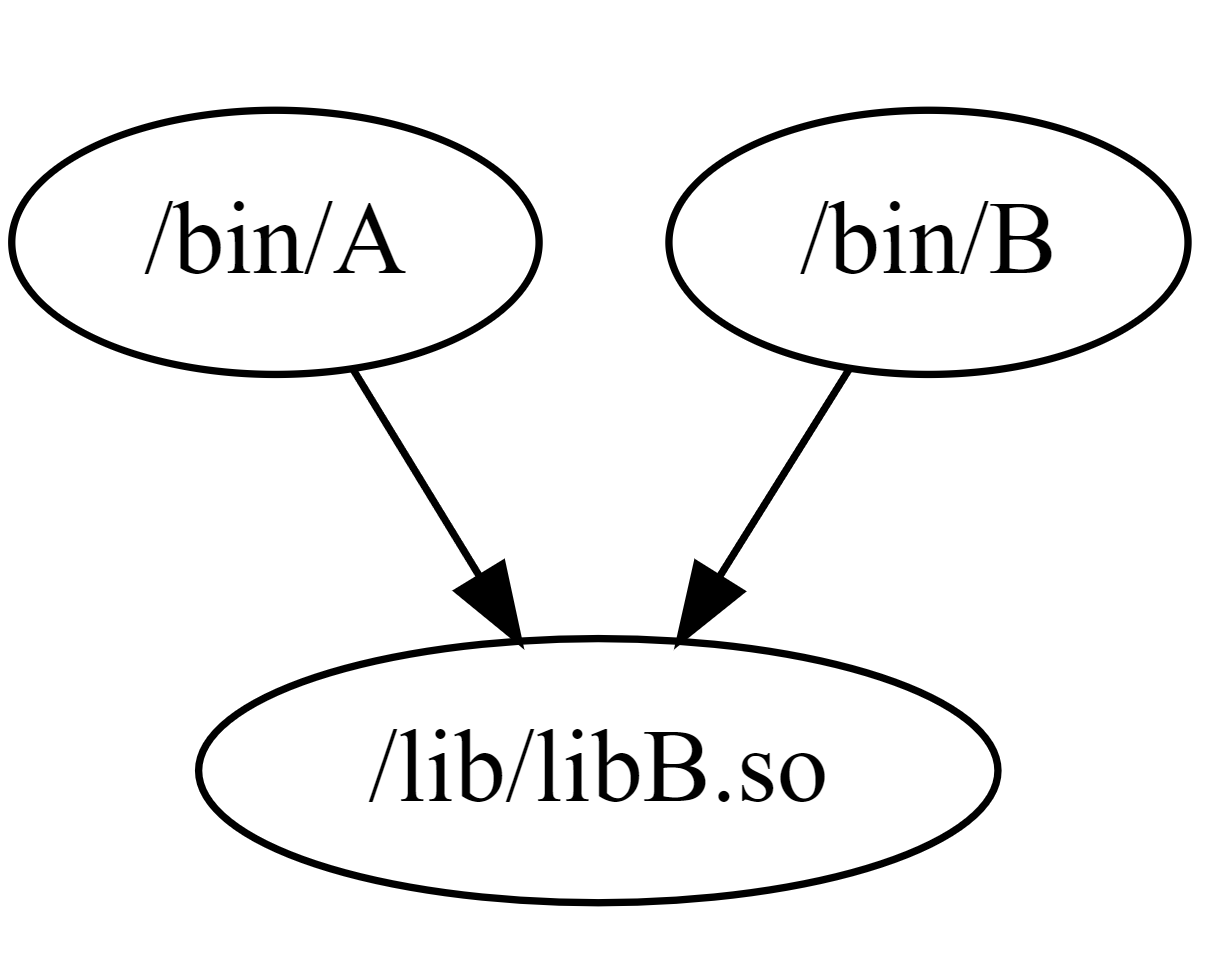
\includegraphics[width=150pt]{Screenshot 2023-05-29 150312.png}
    \caption{Dependency graph of packages A, B and C.}
    \label{fig:graph1}
\end{figure}

This model then couples the dependency graph of the packages, with the structure
of the file system. This means, that not every dependency graph is possible to
be constructed on disk, because we must follow the rules of the file system. For
example, if package |A| wants to use the path |/bin/A|, and package |A'| wants
to use it too, this dependency graph is not possible to be constructed, as we
have a conflict. This is illustrated on figure \ref{fig:graph2}.

\begin{figure}
    \centering
    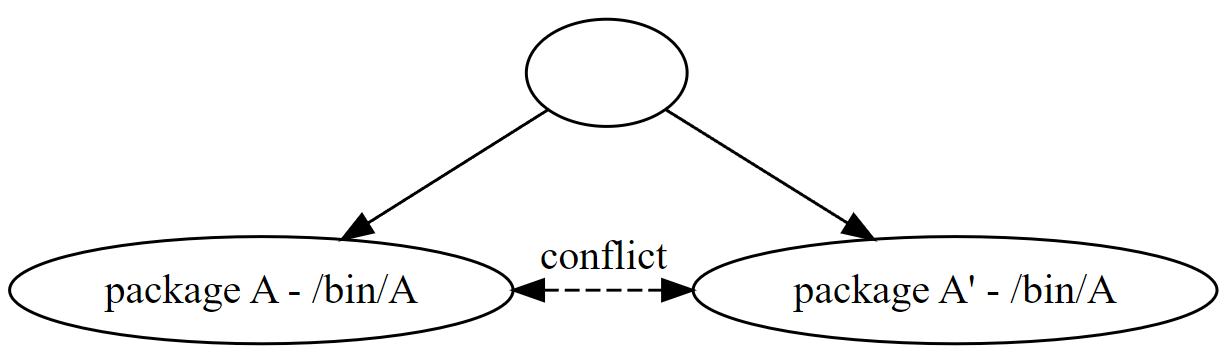
\includegraphics[width=250pt]{Screenshot 2023-05-29 153351.png}
    \caption{Dependency conflict of packages A and A' .}
    \label{fig:graph2}
\end{figure}

A more subtle problem is the Circular Dependency Problem \cite{al-mutawaShapeCircularDependencies2014}. This problem stems
from using an imperative way of managing the dependencies, that is, the usage of
a \ac{CLI} to install or remove packages one after the
other. After requesting some operation on the dependency graph, the result could have
loops in it, as illustrated on figure \ref{fig:graph3}. This causes problems in
the ordering of the operations, and many others. Colloquially, this is known referred to as
``dependency hell'' \cite{abateDependencySolvingStill2020}, denoting the difficulty of managing the dependencies of a system.

\begin{figure}
    \centering
    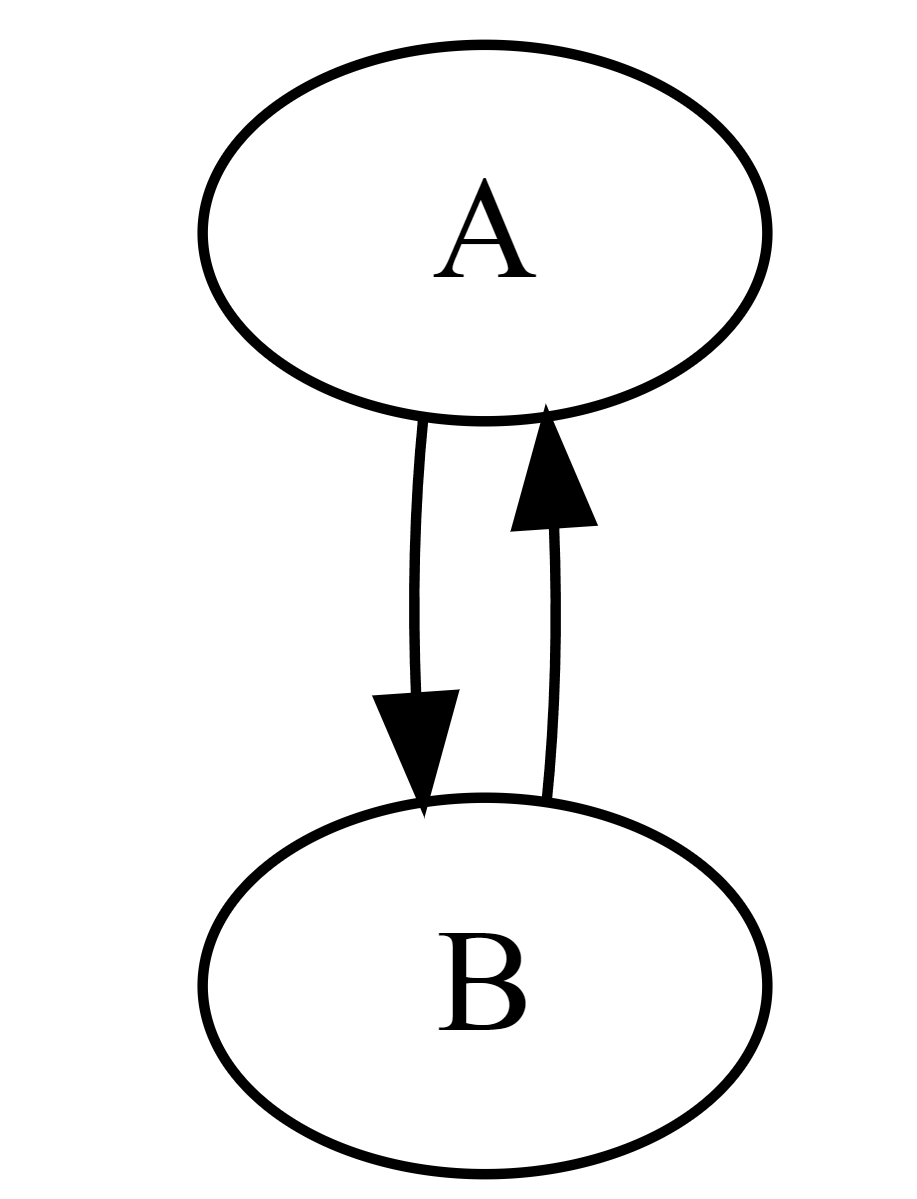
\includegraphics[width=0.2\textwidth]{Screenshot 2023-05-29 154056.png}
    \caption{Circular dependency between A and B.}
    \label{fig:graph3}
\end{figure}

What it is proposed then, is a system where the dependency graph is decoupled
from the file system. This means, that packages don't rely on standard locations
to look for files. Therefore, the \ac{FHS} is not used anymore --- or at least, not
in the same way. The previous work of the Linux distributions
NixOS \cite{dolstraPurelyFunctionalSoftware2006} and Guix System
\cite{courtesFunctionalPackageManagement2013} or Spack, the \ac{HPC} package
manager \cite{gamblinSpackPackageManager2015}, already paved the way into this idea.

In miq (pronounced [miku]), the packages are evaluated into a \ac{DAG}, in which
each node represents a package, and each edge represents a dependency. Then,
each node gets a unique identifier, which depends on its own definition, and the
identifier of its dependencies. This ``identifier'' is represented as a
cryptographic hash. Finally, each package receives a
directory in the file system
unique to its identifier, as shown on figure \ref{fig:graph4}.


\begin{figure}
    \centering
    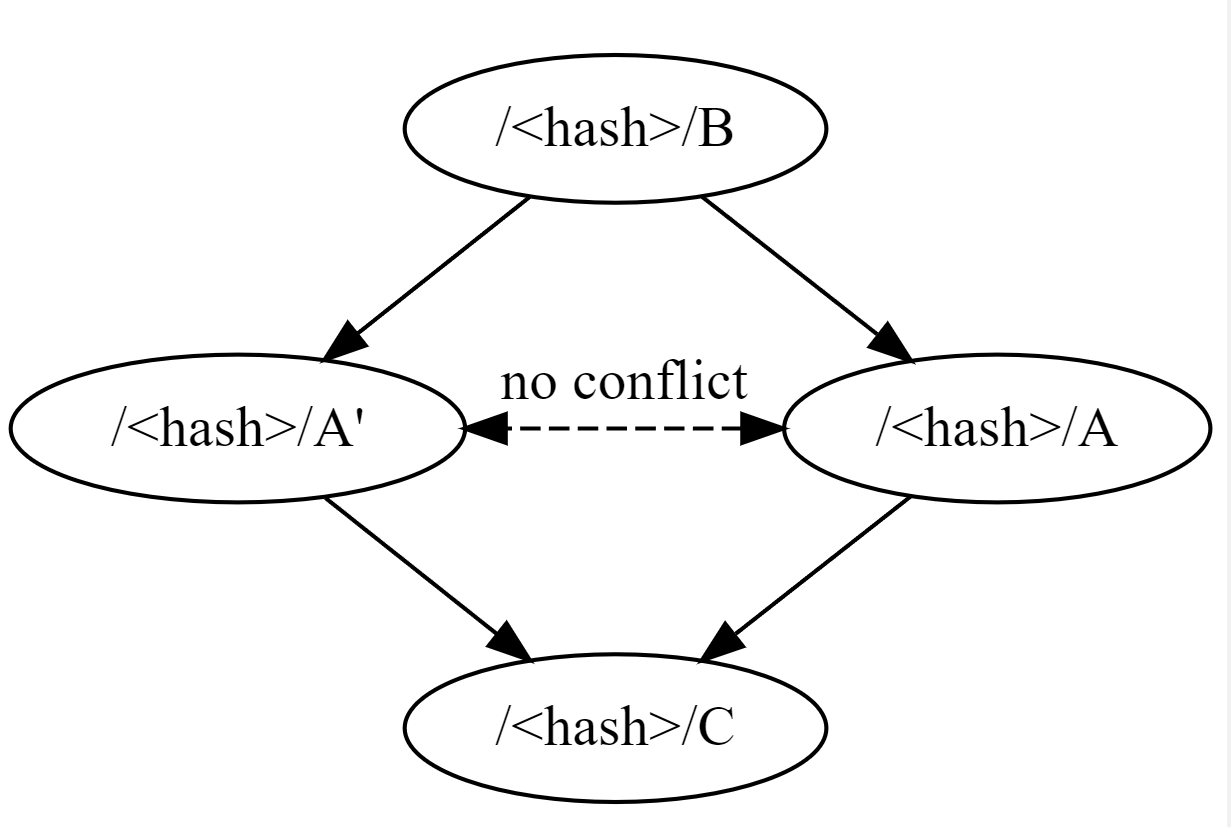
\includegraphics[width=250pt]{Screenshot 2023-05-29 164148.png}
    \caption{Dependency graph of packages A, A', B and C, by using a unique prefix.}
    \label{fig:graph4}
\end{figure}



This system also provides a way to transverse the dependency graph, and look for
any change in the transitive dependency graph. For example, if package |A|
depends on |C| through |B|, a change on |C| triggers a change of its hash. Which
in turns, triggers a change on |B|, and then on |A|. With this system, the full
dependency graph is known. A common problem in Linux is "my application works on
my machine" \cite{mukherjeeFixingDependencyErrors2021}. Even when the application itself is the same, we still rely on
files provided from the system via the \ac{FHS} and the package manager.

Finally, this enables a deployment model where updates don't require modifying
files in place. Traditionally, if we want to update a package with files
|/bin/A| and |/bin/B|, these files are modified in place. This means, that if
there is any problem during the transaction (like a power outage or a disk
failure), the system is left in an inconsistent state. In miq, the original
package would still be available on its old path, and we can delay the update to
just swapping a symlink into the current version.

The main solution to this problem currently is the usage of containers. A
container is a collection of files, which can be thought as Linux distribution
itself \cite{DockerAcceleratedContainerized2022} \cite{merkelDockerLightweightLinux2014}. This container is then run by a ``runtime'', that isolates it from the
host's file system, as shown in figure \ref{fig:graph5} . As a result, the files in the container don't conflict with
the hosts, or other containers. The main way to deploy applications is then
using one container per application, which bundles its entire dependency tree.
Because the underlying file system of each container has the same problems as any
other, the containers solution moves the problem into a singular image, which
contains a single application, and as a result a smaller dependency footprint.

In contrast to miq, where each dependency lives in its own directory, without
collisions and need for a sandboxing runtime, as illustrated in figure
\ref{fig:graph6} .

\begin{figure}[hbt]
    \centering
    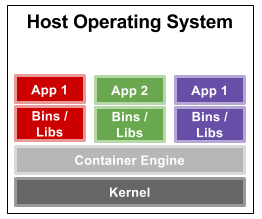
\includegraphics[width=200pt]{Screenshot 2023-05-29 173501.png}
    \caption{Deployment model of containerized applications.}
    \label{fig:graph5}
\end{figure}

\begin{figure}[hbt]
    \centering
    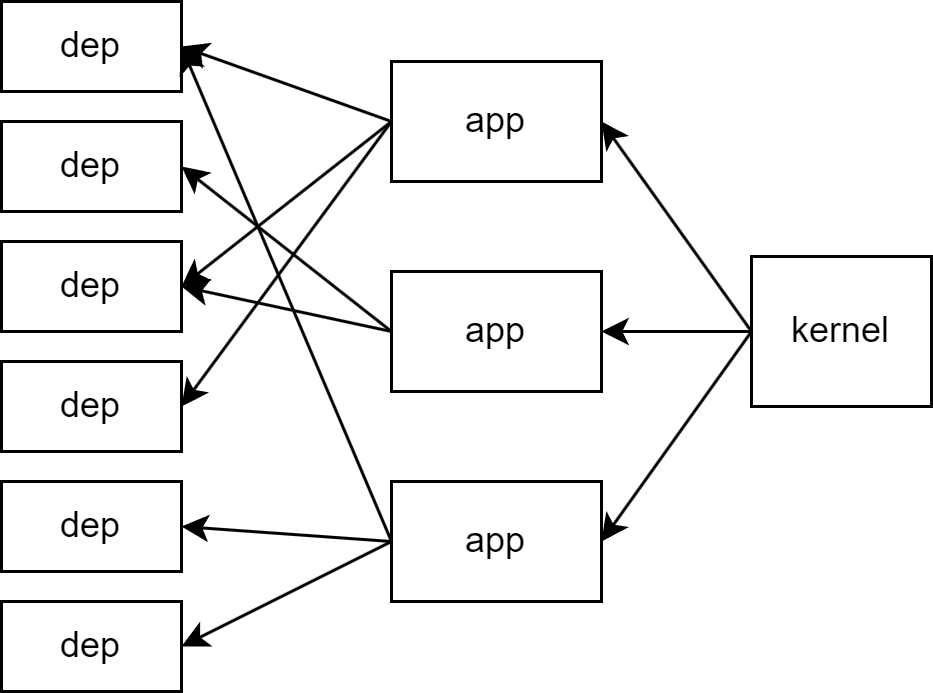
\includegraphics[width=200pt]{dep2.png}
    \caption{Deployment model of miq.}
    \label{fig:graph6}
\end{figure}


